\section{Esempi}
I politopi astratti nascono come assiomatizzazione del pi\`u naturale concetto di politopo concreto al quale siamo abituati, tuttavia questa
assiomatizzazione non caratterizza totalmente i classici politopi dello spazio euclideo, non potendo \emph{imbrigliare} propriet\`a quali
l'assenza di curvatura dei politopi concreti o come la finitezza o ancora propriet\`a pi\`u intrinseche dello spazio euclideo.\\
Per comprendere meglio quali esempi particolari la teoria dei politopi astratti generi o - con un cambio di prospettiva - quali oggetti la
teoria dei politopi concreti scarti, pu\`o venirci in aiuto proprio l'operazione di quoziente tra politopi. Infatti ispirati dagli esempi
concreti dei solidi platonici abbiamo trovato i possibili loro quozienti astratti, per cercare di comprendere meglio se questi possano essere
 visualizzati a mezzo di particolari modelli intuitivi ``concreti''. A tal fine si \`e scritto un software - grazie alla libreria \textsc{sage}
- che caratterizza i quozienti di un politopo dato (che risultino effettivamente politopi), dandone importanti informazioni
 come il gruppo di simmetria con la descrizione della struttura e una presentazione astratta. Inoltre, partendo dai poset cos\`i ottenuti,
 in alcuni casi si \`e proceduto con l'elaborazione di un modello concreto che potesse originare con le proprie relazioni di incidenza
 il politopo astratto trovato, generalizzando in qualche modo l'idea di politopo concreto.
\subsection{Cubo}
Mostriamo i quozienti del cubo che risultano essere ancora politopi. 
%% INIZIO CUBO
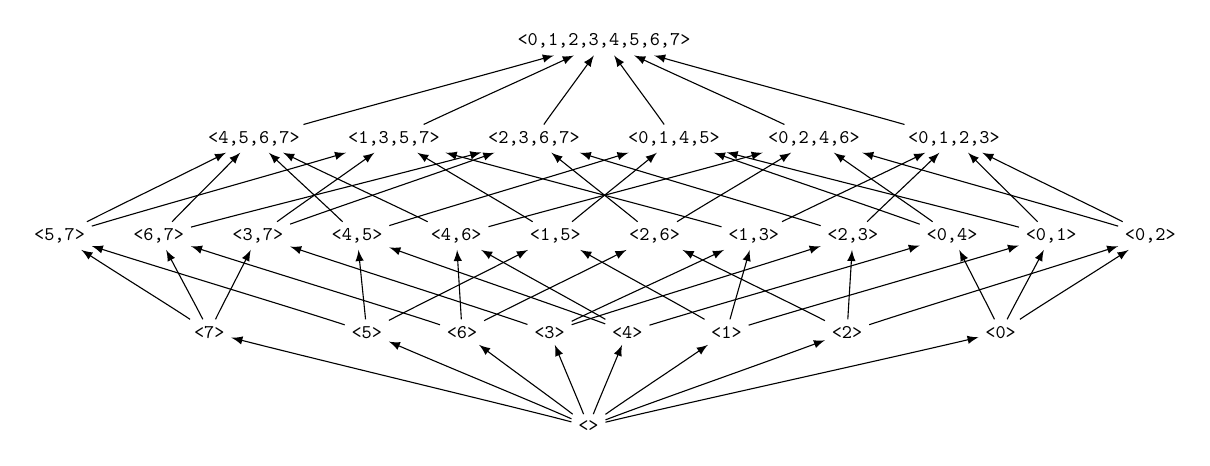
\begin{tikzpicture}[>=latex,line join=bevel,scale=0.700000000000000,every node/.style={scale=0.700000000000000}]
%%
\node (node_26) at (93.5bp,54.5bp) [draw,draw=none] {$\text{\texttt{<7>}}$};
  \node (node_27) at (288.5bp,6.0bp) [draw,draw=none] {$\text{\texttt{<>}}$};
  \node (node_24) at (67.5bp,104.0bp) [draw,draw=none] {$\text{\texttt{<6,7>}}$};
  \node (node_25) at (223.5bp,54.5bp) [draw,draw=none] {$\text{\texttt{<6>}}$};
  \node (node_22) at (16.5bp,104.0bp) [draw,draw=none] {$\text{\texttt{<5,7>}}$};
  \node (node_23) at (174.5bp,54.5bp) [draw,draw=none] {$\text{\texttt{<5>}}$};
  \node (node_20) at (220.5bp,104.0bp) [draw,draw=none] {$\text{\texttt{<4,6>}}$};
  \node (node_21) at (308.5bp,54.5bp) [draw,draw=none] {$\text{\texttt{<4>}}$};
  \node (node_9) at (373.5bp,104.0bp) [draw,draw=none] {$\text{\texttt{<1,3>}}$};
  \node (node_8) at (188.5bp,154.0bp) [draw,draw=none] {$\text{\texttt{<1,3,5,7>}}$};
  \node (node_7) at (500.5bp,54.5bp) [draw,draw=none] {$\text{\texttt{<0>}}$};
  \node (node_6) at (475.5bp,104.0bp) [draw,draw=none] {$\text{\texttt{<0,4>}}$};
  \node (node_5) at (577.5bp,104.0bp) [draw,draw=none] {$\text{\texttt{<0,2>}}$};
  \node (node_4) at (404.5bp,154.0bp) [draw,draw=none] {$\text{\texttt{<0,2,4,6>}}$};
  \node (node_3) at (526.5bp,104.0bp) [draw,draw=none] {$\text{\texttt{<0,1>}}$};
  \node (node_2) at (332.5bp,154.0bp) [draw,draw=none] {$\text{\texttt{<0,1,4,5>}}$};
  \node (node_1) at (476.5bp,154.0bp) [draw,draw=none] {$\text{\texttt{<0,1,2,3>}}$};
  \node (node_0) at (296.5bp,204.0bp) [draw,draw=none] {$\text{\texttt{<0,1,2,3,4,5,6,7>}}$};
  \node (node_19) at (169.5bp,104.0bp) [draw,draw=none] {$\text{\texttt{<4,5>}}$};
  \node (node_18) at (116.5bp,154.0bp) [draw,draw=none] {$\text{\texttt{<4,5,6,7>}}$};
  \node (node_17) at (268.5bp,54.5bp) [draw,draw=none] {$\text{\texttt{<3>}}$};
  \node (node_16) at (118.5bp,104.0bp) [draw,draw=none] {$\text{\texttt{<3,7>}}$};
  \node (node_15) at (421.5bp,54.5bp) [draw,draw=none] {$\text{\texttt{<2>}}$};
  \node (node_14) at (322.5bp,104.0bp) [draw,draw=none] {$\text{\texttt{<2,6>}}$};
  \node (node_13) at (424.5bp,104.0bp) [draw,draw=none] {$\text{\texttt{<2,3>}}$};
  \node (node_12) at (260.5bp,154.0bp) [draw,draw=none] {$\text{\texttt{<2,3,6,7>}}$};
  \node (node_11) at (359.5bp,54.5bp) [draw,draw=none] {$\text{\texttt{<1>}}$};
  \node (node_10) at (271.5bp,104.0bp) [draw,draw=none] {$\text{\texttt{<1,5>}}$};
  \draw [black,->] (node_23) ..controls (201.21bp,68.579bp) and (229.85bp,82.602bp)  .. (node_10);
  \draw [black,->] (node_15) ..controls (394.17bp,68.614bp) and (364.75bp,82.731bp)  .. (node_14);
  \draw [black,->] (node_19) ..controls (213.24bp,117.88bp) and (267.87bp,133.97bp)  .. (node_2);
  \draw [black,->] (node_15) ..controls (457.28bp,66.396bp) and (516.39bp,84.394bp)  .. (node_5);
  \draw [black,->] (node_21) ..controls (284.0bp,68.724bp) and (258.69bp,82.389bp)  .. (node_20);
  \draw [black,->] (node_16) ..controls (159.15bp,118.74bp) and (204.12bp,133.94bp)  .. (node_12);
  \draw [black,->] (node_7) ..controls (521.71bp,68.584bp) and (543.27bp,81.885bp)  .. (node_5);
  \draw [black,->] (node_24) ..controls (81.283bp,118.5bp) and (93.605bp,130.57bp)  .. (node_18);
  \draw [black,->] (node_11) ..controls (396.99bp,66.163bp) and (463.08bp,84.962bp)  .. (node_3);
  \draw [black,->] (node_17) ..controls (304.28bp,66.396bp) and (363.39bp,84.394bp)  .. (node_13);
  \draw [black,->] (node_20) ..controls (190.06bp,119.05bp) and (159.51bp,133.15bp)  .. (node_18);
  \draw [black,->] (node_25) ..controls (222.74bp,67.594bp) and (222.09bp,77.849bp)  .. (node_20);
  \draw [black,->] (node_20) ..controls (267.51bp,117.26bp) and (332.34bp,134.18bp)  .. (node_4);
  \draw [black,->] (node_5) ..controls (532.16bp,117.58bp) and (472.61bp,134.1bp)  .. (node_4);
  \draw [black,->] (node_27) ..controls (250.98bp,15.946bp) and (157.13bp,38.326bp)  .. (node_26);
  \draw [black,->] (node_21) ..controls (275.11bp,66.912bp) and (226.15bp,83.642bp)  .. (node_19);
  \draw [black,->] (node_3) ..controls (512.44bp,118.5bp) and (499.86bp,130.57bp)  .. (node_1);
  \draw [black,->] (node_27) ..controls (283.46bp,18.713bp) and (278.76bp,29.655bp)  .. (node_17);
  \draw [black,->] (node_10) ..controls (288.62bp,118.47bp) and (304.7bp,131.12bp)  .. (node_2);
  \draw [black,->] (node_9) ..controls (326.24bp,117.26bp) and (261.05bp,134.18bp)  .. (node_8);
  \draw [black,->] (node_14) ..controls (346.07bp,118.8bp) and (369.07bp,132.26bp)  .. (node_4);
  \draw [black,->] (node_17) ..controls (233.62bp,66.546bp) and (178.43bp,84.023bp)  .. (node_16);
  \draw [black,->] (node_3) ..controls (478.3bp,116.93bp) and (408.56bp,134.18bp)  .. (node_2);
  \draw [black,->] (node_23) ..controls (138.58bp,66.297bp) and (78.118bp,84.476bp)  .. (node_22);
  \draw [black,->] (node_15) ..controls (422.26bp,67.594bp) and (422.91bp,77.849bp)  .. (node_13);
  \draw [black,->] (node_21) ..controls (345.99bp,66.163bp) and (412.08bp,84.962bp)  .. (node_6);
  \draw [black,->] (node_11) ..controls (335.0bp,68.724bp) and (309.69bp,82.389bp)  .. (node_10);
  \draw [black,->] (node_6) ..controls (455.37bp,118.61bp) and (436.13bp,131.62bp)  .. (node_4);
  \draw [black,->] (node_27) ..controls (293.54bp,18.713bp) and (298.24bp,29.655bp)  .. (node_21);
  \draw [black,->] (node_9) ..controls (403.57bp,119.01bp) and (433.63bp,133.02bp)  .. (node_1);
  \draw [black,->] (node_26) ..controls (86.726bp,67.876bp) and (80.758bp,78.779bp)  .. (node_24);
  \draw [black,->] (node_14) ..controls (305.1bp,118.47bp) and (288.76bp,131.12bp)  .. (node_12);
  \draw [black,->] (node_27) ..controls (327.92bp,15.646bp) and (433.82bp,38.874bp)  .. (node_7);
  \draw [black,->] (node_27) ..controls (271.3bp,19.301bp) and (252.97bp,32.419bp)  .. (node_25);
  \draw [black,->] (node_18) ..controls (170.81bp,169.48bp) and (227.86bp,184.7bp)  .. (node_0);
  \draw [black,->] (node_6) ..controls (434.56bp,118.74bp) and (389.28bp,133.94bp)  .. (node_2);
  \draw [black,->] (node_2) ..controls (322.59bp,168.21bp) and (314.04bp,179.61bp)  .. (node_0);
  \draw [black,->] (node_25) ..controls (187.72bp,66.396bp) and (128.61bp,84.394bp)  .. (node_24);
  \draw [black,->] (node_13) ..controls (380.49bp,117.88bp) and (325.52bp,133.97bp)  .. (node_12);
  \draw [black,->] (node_22) ..controls (61.971bp,117.69bp) and (120.75bp,134.09bp)  .. (node_8);
  \draw [black,->] (node_1) ..controls (422.19bp,169.48bp) and (365.14bp,184.7bp)  .. (node_0);
  \draw [black,->] (node_17) ..controls (296.62bp,68.221bp) and (328.88bp,82.816bp)  .. (node_9);
  \draw [black,->] (node_26) ..controls (100.01bp,67.876bp) and (105.75bp,78.779bp)  .. (node_16);
  \draw [black,->] (node_27) ..controls (307.39bp,19.37bp) and (327.7bp,32.671bp)  .. (node_11);
  \draw [black,->] (node_16) ..controls (138.35bp,118.61bp) and (157.32bp,131.62bp)  .. (node_8);
  \draw [black,->] (node_8) ..controls (220.19bp,169.09bp) and (252.12bp,183.28bp)  .. (node_0);
  \draw [black,->] (node_7) ..controls (493.99bp,67.876bp) and (488.25bp,78.779bp)  .. (node_6);
  \draw [black,->] (node_24) ..controls (115.89bp,117.04bp) and (184.77bp,134.17bp)  .. (node_12);
  \draw [black,->] (node_19) ..controls (154.51bp,118.57bp) and (141.0bp,130.81bp)  .. (node_18);
  \draw [black,->] (node_13) ..controls (439.13bp,118.5bp) and (452.2bp,130.57bp)  .. (node_1);
  \draw [black,->] (node_7) ..controls (507.27bp,67.876bp) and (513.24bp,78.779bp)  .. (node_3);
  \draw [black,->] (node_27) ..controls (318.02bp,17.321bp) and (370.96bp,35.831bp)  .. (node_15);
  \draw [black,->] (node_12) ..controls (270.41bp,168.21bp) and (278.96bp,179.61bp)  .. (node_0);
  \draw [black,->] (node_11) ..controls (363.11bp,67.735bp) and (366.22bp,78.312bp)  .. (node_9);
  \draw [black,->] (node_27) ..controls (262.09bp,17.772bp) and (220.52bp,34.729bp)  .. (node_23);
  \draw [black,->] (node_22) ..controls (45.62bp,118.98bp) and (74.61bp,132.89bp)  .. (node_18);
  \draw [black,->] (node_5) ..controls (548.01bp,119.01bp) and (518.54bp,133.02bp)  .. (node_1);
  \draw [black,->] (node_10) ..controls (247.64bp,118.8bp) and (224.36bp,132.26bp)  .. (node_8);
  \draw [black,->] (node_26) ..controls (72.29bp,68.584bp) and (50.729bp,81.885bp)  .. (node_22);
  \draw [black,->] (node_23) ..controls (173.23bp,67.594bp) and (172.15bp,77.849bp)  .. (node_19);
  \draw [black,->] (node_4) ..controls (372.81bp,169.09bp) and (340.88bp,183.28bp)  .. (node_0);
  \draw [black,->] (node_25) ..controls (250.83bp,68.614bp) and (280.25bp,82.731bp)  .. (node_14);
%
\end{tikzpicture}\\
\textsc{Sottogruppo identico}\\
Vettore delle facce: $(1, 8, 12, 6, 1)$\\
Politopo\ \textbf{regolare}\\
Simbolo di Shlafli: $\{4, 3\}$\\
\textbf{Gruppo}:\\Presentazione: $< a, b, c | a^2, c^2, b^2, (c*a)^2, (b*c)^3, (b*a)^4 >$\\
Struttura: $C2 x S4$\\
\newpage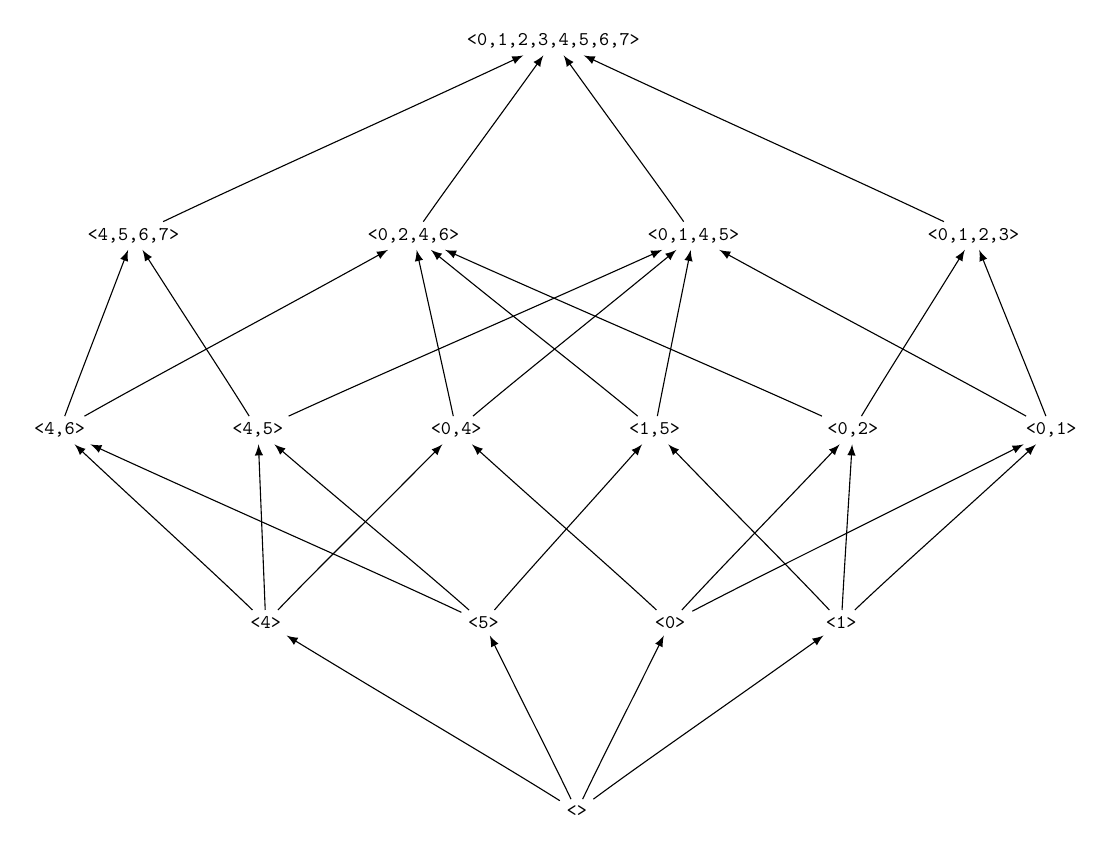
\begin{tikzpicture}[>=latex,line join=bevel,scale=1.40000000000000,every node/.style={scale=0.700000000000000}]
%%
\node (node_13) at (69.5bp,54.5bp) [draw,draw=none] {$\text{\texttt{<4>}}$};
  \node (node_14) at (125.5bp,54.5bp) [draw,draw=none] {$\text{\texttt{<5>}}$};
  \node (node_9) at (217.5bp,54.5bp) [draw,draw=none] {$\text{\texttt{<1>}}$};
  \node (node_8) at (169.5bp,104.0bp) [draw,draw=none] {$\text{\texttt{<1,5>}}$};
  \node (node_7) at (173.5bp,54.5bp) [draw,draw=none] {$\text{\texttt{<0>}}$};
  \node (node_6) at (118.5bp,104.0bp) [draw,draw=none] {$\text{\texttt{<0,4>}}$};
  \node (node_5) at (220.5bp,104.0bp) [draw,draw=none] {$\text{\texttt{<0,2>}}$};
  \node (node_4) at (107.5bp,154.0bp) [draw,draw=none] {$\text{\texttt{<0,2,4,6>}}$};
  \node (node_3) at (271.5bp,104.0bp) [draw,draw=none] {$\text{\texttt{<0,1>}}$};
  \node (node_2) at (179.5bp,154.0bp) [draw,draw=none] {$\text{\texttt{<0,1,4,5>}}$};
  \node (node_1) at (251.5bp,154.0bp) [draw,draw=none] {$\text{\texttt{<0,1,2,3>}}$};
  \node (node_10) at (35.5bp,154.0bp) [draw,draw=none] {$\text{\texttt{<4,5,6,7>}}$};
  \node (node_11) at (67.5bp,104.0bp) [draw,draw=none] {$\text{\texttt{<4,5>}}$};
  \node (node_0) at (143.5bp,204.0bp) [draw,draw=none] {$\text{\texttt{<0,1,2,3,4,5,6,7>}}$};
  \node (node_15) at (149.5bp,6.0bp) [draw,draw=none] {$\text{\texttt{<>}}$};
  \node (node_12) at (16.5bp,104.0bp) [draw,draw=none] {$\text{\texttt{<4,6>}}$};
  \draw [black,->] (node_14) ..controls (137.29bp,68.228bp) and (148.16bp,79.964bp)  .. (node_8);
  \draw [black,->] (node_15) ..controls (167.59bp,19.37bp) and (187.04bp,32.671bp)  .. (node_9);
  \draw [black,->] (node_5) ..controls (187.25bp,119.12bp) and (153.63bp,133.4bp)  .. (node_4);
  \draw [black,->] (node_15) ..controls (128.34bp,19.301bp) and (104.49bp,33.163bp)  .. (node_13);
  \draw [black,->] (node_7) ..controls (158.52bp,68.44bp) and (144.34bp,80.687bp)  .. (node_6);
  \draw [black,->] (node_11) ..controls (58.74bp,118.14bp) and (51.248bp,129.38bp)  .. (node_10);
  \draw [black,->] (node_14) ..controls (109.61bp,68.51bp) and (94.449bp,80.93bp)  .. (node_11);
  \draw [black,->] (node_8) ..controls (152.1bp,118.47bp) and (135.76bp,131.12bp)  .. (node_4);
  \draw [black,->] (node_13) ..controls (68.991bp,67.594bp) and (68.559bp,77.849bp)  .. (node_11);
  \draw [black,->] (node_9) ..controls (204.5bp,68.369bp) and (192.29bp,80.445bp)  .. (node_8);
  \draw [black,->] (node_3) ..controls (244.85bp,118.91bp) and (218.52bp,132.64bp)  .. (node_2);
  \draw [black,->] (node_9) ..controls (218.26bp,67.594bp) and (218.91bp,77.849bp)  .. (node_5);
  \draw [black,->] (node_7) ..controls (186.16bp,68.299bp) and (197.94bp,80.204bp)  .. (node_5);
  \draw [black,->] (node_11) ..controls (100.37bp,119.09bp) and (133.48bp,133.28bp)  .. (node_2);
  \draw [black,->] (node_15) ..controls (143.42bp,18.782bp) and (137.68bp,29.894bp)  .. (node_14);
  \draw [black,->] (node_6) ..controls (115.57bp,117.78bp) and (113.18bp,128.21bp)  .. (node_4);
  \draw [black,->] (node_13) ..controls (82.776bp,68.369bp) and (95.233bp,80.445bp)  .. (node_6);
  \draw [black,->] (node_14) ..controls (96.809bp,68.003bp) and (62.89bp,82.784bp)  .. (node_12);
  \draw [black,->] (node_15) ..controls (155.58bp,18.782bp) and (161.32bp,29.894bp)  .. (node_7);
  \draw [black,->] (node_2) ..controls (169.59bp,168.21bp) and (161.04bp,179.61bp)  .. (node_0);
  \draw [black,->] (node_3) ..controls (266.12bp,117.92bp) and (261.64bp,128.67bp)  .. (node_1);
  \draw [black,->] (node_12) ..controls (21.587bp,117.85bp) and (25.778bp,128.44bp)  .. (node_10);
  \draw [black,->] (node_1) ..controls (219.81bp,169.09bp) and (187.88bp,183.28bp)  .. (node_0);
  \draw [black,->] (node_9) ..controls (232.21bp,68.44bp) and (246.13bp,80.687bp)  .. (node_3);
  \draw [black,->] (node_10) ..controls (67.193bp,169.09bp) and (99.119bp,183.28bp)  .. (node_0);
  \draw [black,->] (node_12) ..controls (42.794bp,118.87bp) and (68.66bp,132.51bp)  .. (node_4);
  \draw [black,->] (node_6) ..controls (135.62bp,118.47bp) and (151.7bp,131.12bp)  .. (node_2);
  \draw [black,->] (node_7) ..controls (200.56bp,68.614bp) and (229.68bp,82.731bp)  .. (node_3);
  \draw [black,->] (node_8) ..controls (172.16bp,117.78bp) and (174.33bp,128.21bp)  .. (node_2);
  \draw [black,->] (node_13) ..controls (55.062bp,68.44bp) and (41.397bp,80.687bp)  .. (node_12);
  \draw [black,->] (node_5) ..controls (228.99bp,118.14bp) and (236.24bp,129.38bp)  .. (node_1);
  \draw [black,->] (node_4) ..controls (117.41bp,168.21bp) and (125.96bp,179.61bp)  .. (node_0);
%
\end{tikzpicture}\\
\textsc{Sottogruppo generato da: }$(<0>, <3>)(<1>, <2>)(<4>, <7>)(<5>, <6>)$\\
\\
Vettore delle facce: $(1, 4, 6, 4, 1)$\\
\textbf{Gruppo}:\\Presentazione: $< a, b, c | a^2, b^2, c^2, (c*b)^2, (c*a)^2, (b*a)^2 >$\\
Struttura: $C2 x C2 x C2$\\
\newpage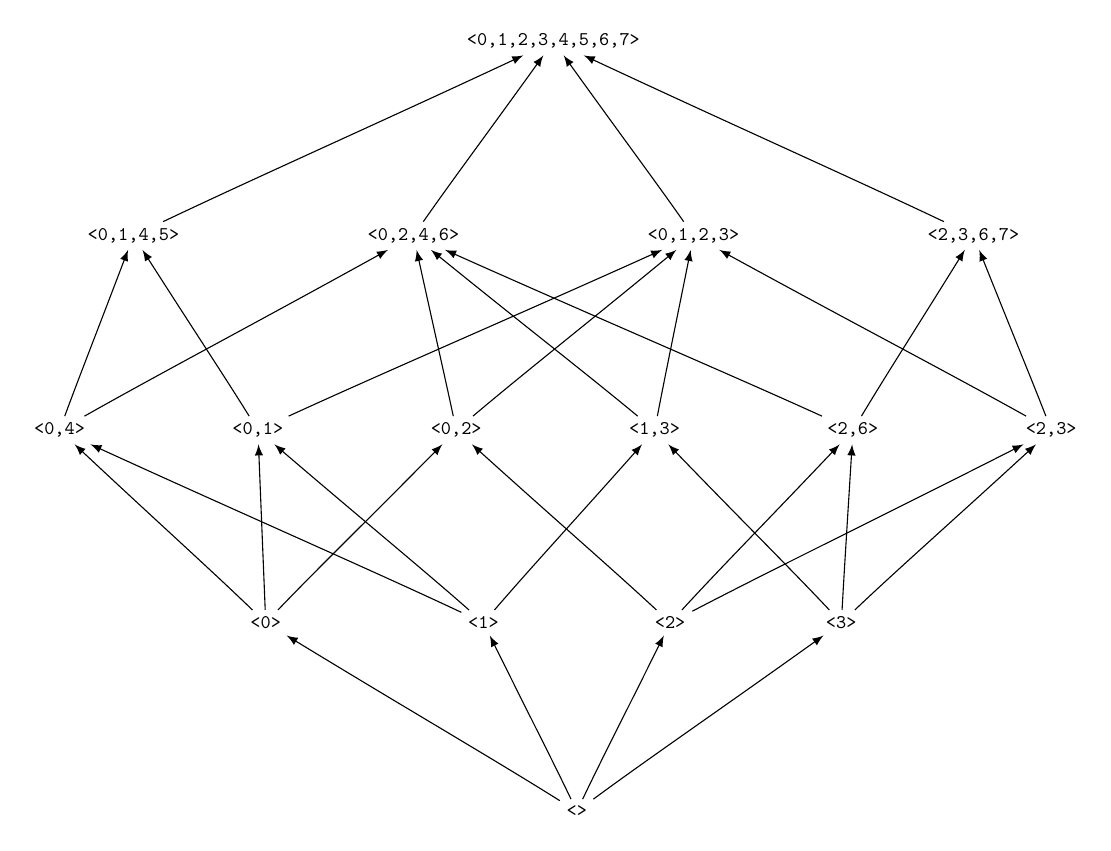
\begin{tikzpicture}[>=latex,line join=bevel,scale=1.40000000000000,every node/.style={scale=0.700000000000000}]
%%
\node (node_13) at (173.5bp,54.5bp) [draw,draw=none] {$\text{\texttt{<2>}}$};
  \node (node_4) at (107.5bp,154.0bp) [draw,draw=none] {$\text{\texttt{<0,2,4,6>}}$};
  \node (node_9) at (125.5bp,54.5bp) [draw,draw=none] {$\text{\texttt{<1>}}$};
  \node (node_8) at (169.5bp,104.0bp) [draw,draw=none] {$\text{\texttt{<1,3>}}$};
  \node (node_7) at (69.5bp,54.5bp) [draw,draw=none] {$\text{\texttt{<0>}}$};
  \node (node_6) at (16.5bp,104.0bp) [draw,draw=none] {$\text{\texttt{<0,4>}}$};
  \node (node_5) at (118.5bp,104.0bp) [draw,draw=none] {$\text{\texttt{<0,2>}}$};
  \node (node_14) at (217.5bp,54.5bp) [draw,draw=none] {$\text{\texttt{<3>}}$};
  \node (node_3) at (67.5bp,104.0bp) [draw,draw=none] {$\text{\texttt{<0,1>}}$};
  \node (node_2) at (35.5bp,154.0bp) [draw,draw=none] {$\text{\texttt{<0,1,4,5>}}$};
  \node (node_1) at (179.5bp,154.0bp) [draw,draw=none] {$\text{\texttt{<0,1,2,3>}}$};
  \node (node_10) at (251.5bp,154.0bp) [draw,draw=none] {$\text{\texttt{<2,3,6,7>}}$};
  \node (node_11) at (271.5bp,104.0bp) [draw,draw=none] {$\text{\texttt{<2,3>}}$};
  \node (node_0) at (143.5bp,204.0bp) [draw,draw=none] {$\text{\texttt{<0,1,2,3,4,5,6,7>}}$};
  \node (node_15) at (149.5bp,6.0bp) [draw,draw=none] {$\text{\texttt{<>}}$};
  \node (node_12) at (220.5bp,104.0bp) [draw,draw=none] {$\text{\texttt{<2,6>}}$};
  \draw [black,->] (node_14) ..controls (204.5bp,68.369bp) and (192.29bp,80.445bp)  .. (node_8);
  \draw [black,->] (node_9) ..controls (96.809bp,68.003bp) and (62.89bp,82.784bp)  .. (node_6);
  \draw [black,->] (node_5) ..controls (115.57bp,117.78bp) and (113.18bp,128.21bp)  .. (node_4);
  \draw [black,->] (node_13) ..controls (158.52bp,68.44bp) and (144.34bp,80.687bp)  .. (node_5);
  \draw [black,->] (node_15) ..controls (155.58bp,18.782bp) and (161.32bp,29.894bp)  .. (node_13);
  \draw [black,->] (node_7) ..controls (55.062bp,68.44bp) and (41.397bp,80.687bp)  .. (node_6);
  \draw [black,->] (node_11) ..controls (266.12bp,117.92bp) and (261.64bp,128.67bp)  .. (node_10);
  \draw [black,->] (node_14) ..controls (232.21bp,68.44bp) and (246.13bp,80.687bp)  .. (node_11);
  \draw [black,->] (node_8) ..controls (152.1bp,118.47bp) and (135.76bp,131.12bp)  .. (node_4);
  \draw [black,->] (node_15) ..controls (167.59bp,19.37bp) and (187.04bp,32.671bp)  .. (node_14);
  \draw [black,->] (node_13) ..controls (200.56bp,68.614bp) and (229.68bp,82.731bp)  .. (node_11);
  \draw [black,->] (node_9) ..controls (137.29bp,68.228bp) and (148.16bp,79.964bp)  .. (node_8);
  \draw [black,->] (node_3) ..controls (58.74bp,118.14bp) and (51.248bp,129.38bp)  .. (node_2);
  \draw [black,->] (node_15) ..controls (143.42bp,18.782bp) and (137.68bp,29.894bp)  .. (node_9);
  \draw [black,->] (node_7) ..controls (82.776bp,68.369bp) and (95.233bp,80.445bp)  .. (node_5);
  \draw [black,->] (node_6) ..controls (42.794bp,118.87bp) and (68.66bp,132.51bp)  .. (node_4);
  \draw [black,->] (node_14) ..controls (218.26bp,67.594bp) and (218.91bp,77.849bp)  .. (node_12);
  \draw [black,->] (node_15) ..controls (128.34bp,19.301bp) and (104.49bp,33.163bp)  .. (node_7);
  \draw [black,->] (node_8) ..controls (172.16bp,117.78bp) and (174.33bp,128.21bp)  .. (node_1);
  \draw [black,->] (node_12) ..controls (228.99bp,118.14bp) and (236.24bp,129.38bp)  .. (node_10);
  \draw [black,->] (node_3) ..controls (100.37bp,119.09bp) and (133.48bp,133.28bp)  .. (node_1);
  \draw [black,->] (node_2) ..controls (67.193bp,169.09bp) and (99.119bp,183.28bp)  .. (node_0);
  \draw [black,->] (node_1) ..controls (169.59bp,168.21bp) and (161.04bp,179.61bp)  .. (node_0);
  \draw [black,->] (node_11) ..controls (244.85bp,118.91bp) and (218.52bp,132.64bp)  .. (node_1);
  \draw [black,->] (node_9) ..controls (109.61bp,68.51bp) and (94.449bp,80.93bp)  .. (node_3);
  \draw [black,->] (node_10) ..controls (219.81bp,169.09bp) and (187.88bp,183.28bp)  .. (node_0);
  \draw [black,->] (node_12) ..controls (187.25bp,119.12bp) and (153.63bp,133.4bp)  .. (node_4);
  \draw [black,->] (node_6) ..controls (21.587bp,117.85bp) and (25.778bp,128.44bp)  .. (node_2);
  \draw [black,->] (node_7) ..controls (68.991bp,67.594bp) and (68.559bp,77.849bp)  .. (node_3);
  \draw [black,->] (node_13) ..controls (186.16bp,68.299bp) and (197.94bp,80.204bp)  .. (node_12);
  \draw [black,->] (node_5) ..controls (135.62bp,118.47bp) and (151.7bp,131.12bp)  .. (node_1);
  \draw [black,->] (node_4) ..controls (117.41bp,168.21bp) and (125.96bp,179.61bp)  .. (node_0);
%
\end{tikzpicture}\\
\textsc{Sottogruppo generato da: }$(<0>, <5>)(<1>, <4>)(<2>, <7>)(<3>, <6>)$\\
\\
Vettore delle facce: $(1, 4, 6, 4, 1)$\\
\textbf{Gruppo}:\\Presentazione: $< a, b, c | a^2, b^2, c^2, (c*b)^2, (c*a)^2, (b*a)^2 >$\\
Struttura: $C2 x C2 x C2$\\
\newpage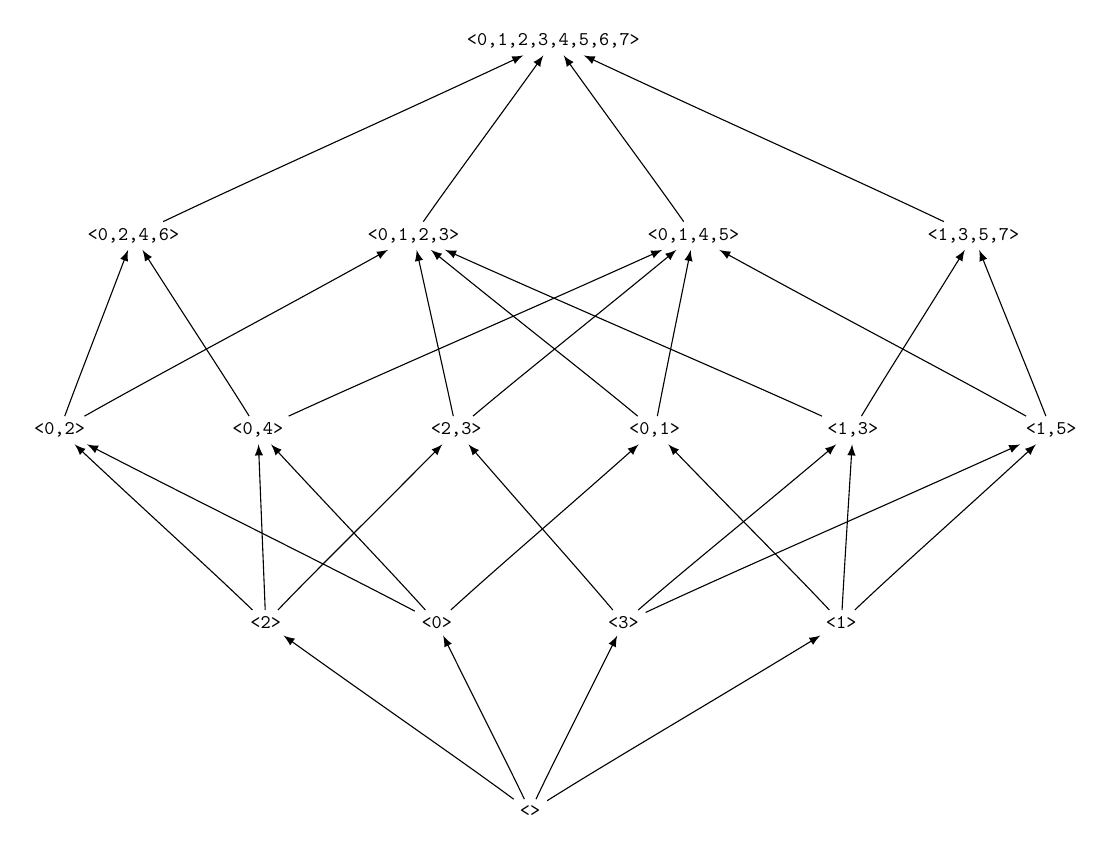
\begin{tikzpicture}[>=latex,line join=bevel,scale=1.40000000000000,every node/.style={scale=0.700000000000000}]
%%
\node (node_13) at (69.5bp,54.5bp) [draw,draw=none] {$\text{\texttt{<2>}}$};
  \node (node_4) at (35.5bp,154.0bp) [draw,draw=none] {$\text{\texttt{<0,2,4,6>}}$};
  \node (node_9) at (220.5bp,104.0bp) [draw,draw=none] {$\text{\texttt{<1,3>}}$};
  \node (node_8) at (251.5bp,154.0bp) [draw,draw=none] {$\text{\texttt{<1,3,5,7>}}$};
  \node (node_7) at (113.5bp,54.5bp) [draw,draw=none] {$\text{\texttt{<0>}}$};
  \node (node_6) at (67.5bp,104.0bp) [draw,draw=none] {$\text{\texttt{<0,4>}}$};
  \node (node_5) at (16.5bp,104.0bp) [draw,draw=none] {$\text{\texttt{<0,2>}}$};
  \node (node_14) at (161.5bp,54.5bp) [draw,draw=none] {$\text{\texttt{<3>}}$};
  \node (node_3) at (169.5bp,104.0bp) [draw,draw=none] {$\text{\texttt{<0,1>}}$};
  \node (node_12) at (118.5bp,104.0bp) [draw,draw=none] {$\text{\texttt{<2,3>}}$};
  \node (node_1) at (107.5bp,154.0bp) [draw,draw=none] {$\text{\texttt{<0,1,2,3>}}$};
  \node (node_2) at (179.5bp,154.0bp) [draw,draw=none] {$\text{\texttt{<0,1,4,5>}}$};
  \node (node_10) at (271.5bp,104.0bp) [draw,draw=none] {$\text{\texttt{<1,5>}}$};
  \node (node_11) at (217.5bp,54.5bp) [draw,draw=none] {$\text{\texttt{<1>}}$};
  \node (node_0) at (143.5bp,204.0bp) [draw,draw=none] {$\text{\texttt{<0,1,2,3,4,5,6,7>}}$};
  \node (node_15) at (137.5bp,6.0bp) [draw,draw=none] {$\text{\texttt{<>}}$};
  \draw [black,->] (node_15) ..controls (143.58bp,18.782bp) and (149.32bp,29.894bp)  .. (node_14);
  \draw [black,->] (node_12) ..controls (115.57bp,117.78bp) and (113.18bp,128.21bp)  .. (node_1);
  \draw [black,->] (node_15) ..controls (119.41bp,19.37bp) and (99.959bp,32.671bp)  .. (node_13);
  \draw [black,->] (node_7) ..controls (101.11bp,68.299bp) and (89.576bp,80.204bp)  .. (node_6);
  \draw [black,->] (node_11) ..controls (204.5bp,68.369bp) and (192.29bp,80.445bp)  .. (node_3);
  \draw [black,->] (node_11) ..controls (232.21bp,68.44bp) and (246.13bp,80.687bp)  .. (node_10);
  \draw [black,->] (node_5) ..controls (21.587bp,117.85bp) and (25.778bp,128.44bp)  .. (node_4);
  \draw [black,->] (node_14) ..controls (177.66bp,68.51bp) and (193.09bp,80.93bp)  .. (node_9);
  \draw [black,->] (node_9) ..controls (187.25bp,119.12bp) and (153.63bp,133.4bp)  .. (node_1);
  \draw [black,->] (node_10) ..controls (244.85bp,118.91bp) and (218.52bp,132.64bp)  .. (node_2);
  \draw [black,->] (node_9) ..controls (228.99bp,118.14bp) and (236.24bp,129.38bp)  .. (node_8);
  \draw [black,->] (node_12) ..controls (135.62bp,118.47bp) and (151.7bp,131.12bp)  .. (node_2);
  \draw [black,->] (node_3) ..controls (172.16bp,117.78bp) and (174.33bp,128.21bp)  .. (node_2);
  \draw [black,->] (node_7) ..controls (86.792bp,68.579bp) and (58.154bp,82.602bp)  .. (node_5);
  \draw [black,->] (node_6) ..controls (58.74bp,118.14bp) and (51.248bp,129.38bp)  .. (node_4);
  \draw [black,->] (node_13) ..controls (68.991bp,67.594bp) and (68.559bp,77.849bp)  .. (node_6);
  \draw [black,->] (node_14) ..controls (149.98bp,68.228bp) and (139.35bp,79.964bp)  .. (node_12);
  \draw [black,->] (node_15) ..controls (131.42bp,18.782bp) and (125.68bp,29.894bp)  .. (node_7);
  \draw [black,->] (node_3) ..controls (152.1bp,118.47bp) and (135.76bp,131.12bp)  .. (node_1);
  \draw [black,->] (node_2) ..controls (169.59bp,168.21bp) and (161.04bp,179.61bp)  .. (node_0);
  \draw [black,->] (node_1) ..controls (117.41bp,168.21bp) and (125.96bp,179.61bp)  .. (node_0);
  \draw [black,->] (node_14) ..controls (190.45bp,68.003bp) and (224.68bp,82.784bp)  .. (node_10);
  \draw [black,->] (node_13) ..controls (55.062bp,68.44bp) and (41.397bp,80.687bp)  .. (node_5);
  \draw [black,->] (node_8) ..controls (219.81bp,169.09bp) and (187.88bp,183.28bp)  .. (node_0);
  \draw [black,->] (node_6) ..controls (100.37bp,119.09bp) and (133.48bp,133.28bp)  .. (node_2);
  \draw [black,->] (node_7) ..controls (128.84bp,68.51bp) and (143.48bp,80.93bp)  .. (node_3);
  \draw [black,->] (node_11) ..controls (218.26bp,67.594bp) and (218.91bp,77.849bp)  .. (node_9);
  \draw [black,->] (node_13) ..controls (82.776bp,68.369bp) and (95.233bp,80.445bp)  .. (node_12);
  \draw [black,->] (node_15) ..controls (158.66bp,19.301bp) and (182.51bp,33.163bp)  .. (node_11);
  \draw [black,->] (node_10) ..controls (266.12bp,117.92bp) and (261.64bp,128.67bp)  .. (node_8);
  \draw [black,->] (node_5) ..controls (42.794bp,118.87bp) and (68.66bp,132.51bp)  .. (node_1);
  \draw [black,->] (node_4) ..controls (67.193bp,169.09bp) and (99.119bp,183.28bp)  .. (node_0);
%
\end{tikzpicture}\\
\textsc{Sottogruppo generato da: }$(<0>, <6>)(<1>, <7>)(<2>, <4>)(<3>, <5>)$\\
\\
Vettore delle facce: $(1, 4, 6, 4, 1)$\\
\textbf{Gruppo}:\\Presentazione: $< a, b, c | a^2, b^2, c^2, (c*b)^2, (c*a)^2, (b*a)^2 >$\\
Struttura: $C2 x C2 x C2$\\
\newpage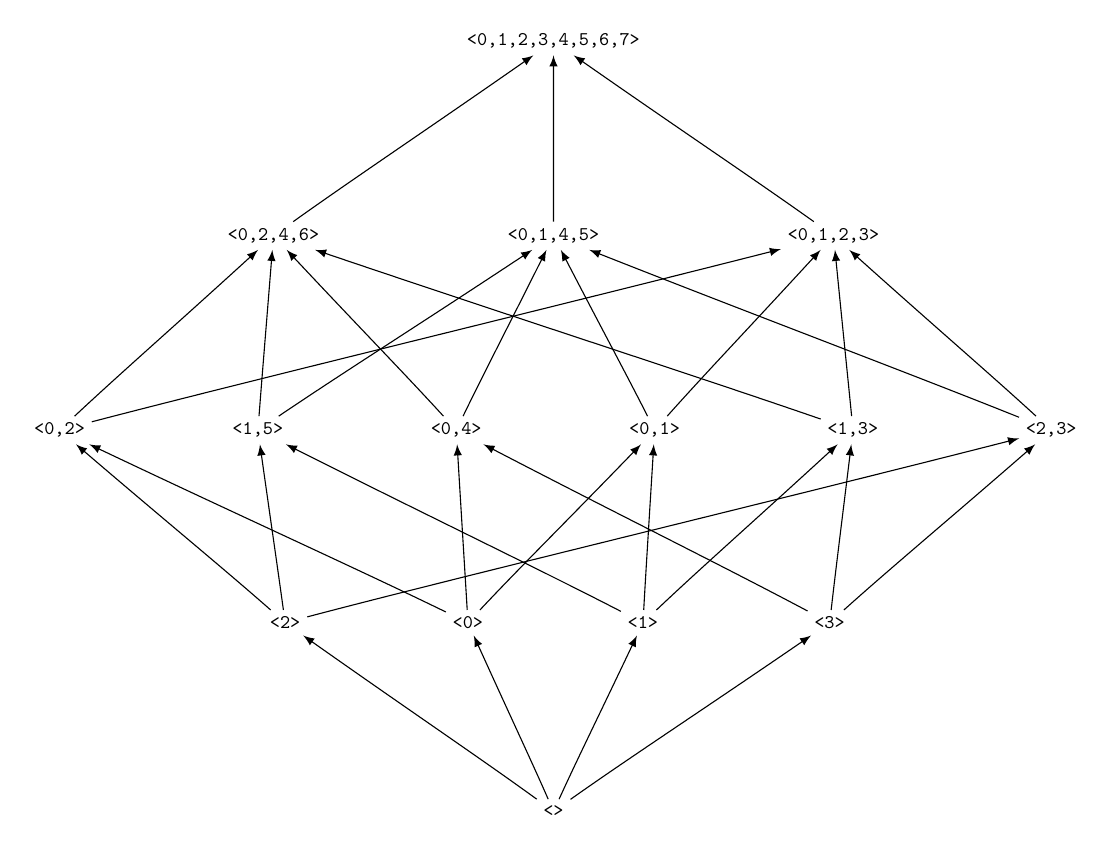
\begin{tikzpicture}[>=latex,line join=bevel,scale=1.40000000000000,every node/.style={scale=0.700000000000000}]
%%
\node (node_13) at (214.5bp,54.5bp) [draw,draw=none] {$\text{\texttt{<3>}}$};
  \node (node_4) at (71.5bp,154.0bp) [draw,draw=none] {$\text{\texttt{<0,2,4,6>}}$};
  \node (node_9) at (67.5bp,104.0bp) [draw,draw=none] {$\text{\texttt{<1,5>}}$};
  \node (node_8) at (220.5bp,104.0bp) [draw,draw=none] {$\text{\texttt{<1,3>}}$};
  \node (node_7) at (121.5bp,54.5bp) [draw,draw=none] {$\text{\texttt{<0>}}$};
  \node (node_6) at (118.5bp,104.0bp) [draw,draw=none] {$\text{\texttt{<0,4>}}$};
  \node (node_5) at (16.5bp,104.0bp) [draw,draw=none] {$\text{\texttt{<0,2>}}$};
  \node (node_14) at (143.5bp,6.0bp) [draw,draw=none] {$\text{\texttt{<>}}$};
  \node (node_3) at (169.5bp,104.0bp) [draw,draw=none] {$\text{\texttt{<0,1>}}$};
  \node (node_2) at (143.5bp,154.0bp) [draw,draw=none] {$\text{\texttt{<0,1,4,5>}}$};
  \node (node_1) at (215.5bp,154.0bp) [draw,draw=none] {$\text{\texttt{<0,1,2,3>}}$};
  \node (node_10) at (166.5bp,54.5bp) [draw,draw=none] {$\text{\texttt{<1>}}$};
  \node (node_11) at (271.5bp,104.0bp) [draw,draw=none] {$\text{\texttt{<2,3>}}$};
  \node (node_0) at (143.5bp,204.0bp) [draw,draw=none] {$\text{\texttt{<0,1,2,3,4,5,6,7>}}$};
  \node (node_12) at (74.5bp,54.5bp) [draw,draw=none] {$\text{\texttt{<2>}}$};
  \draw [black,->] (node_5) ..controls (32.054bp,118.57bp) and (46.079bp,130.81bp)  .. (node_4);
  \draw [black,->] (node_14) ..controls (137.96bp,18.713bp) and (132.78bp,29.655bp)  .. (node_7);
  \draw [black,->] (node_7) ..controls (120.74bp,67.594bp) and (120.09bp,77.849bp)  .. (node_6);
  \draw [black,->] (node_10) ..controls (139.17bp,68.614bp) and (109.75bp,82.731bp)  .. (node_9);
  \draw [black,->] (node_8) ..controls (178.93bp,118.39bp) and (130.99bp,133.84bp)  .. (node_4);
  \draw [black,->] (node_3) ..controls (182.37bp,118.43bp) and (193.78bp,130.33bp)  .. (node_1);
  \draw [black,->] (node_3) ..controls (162.46bp,118.0bp) and (156.55bp,128.91bp)  .. (node_2);
  \draw [black,->] (node_7) ..controls (93.38bp,68.221bp) and (61.117bp,82.816bp)  .. (node_5);
  \draw [black,->] (node_11) ..controls (233.55bp,119.23bp) and (194.73bp,133.79bp)  .. (node_2);
  \draw [black,->] (node_6) ..controls (105.35bp,118.43bp) and (93.696bp,130.33bp)  .. (node_4);
  \draw [black,->] (node_13) ..controls (188.07bp,68.579bp) and (159.72bp,82.602bp)  .. (node_6);
  \draw [black,->] (node_14) ..controls (125.14bp,19.37bp) and (105.41bp,32.671bp)  .. (node_12);
  \draw [black,->] (node_10) ..controls (167.26bp,67.594bp) and (167.91bp,77.849bp)  .. (node_3);
  \draw [black,->] (node_8) ..controls (219.18bp,117.71bp) and (218.11bp,127.98bp)  .. (node_1);
  \draw [black,->] (node_13) ..controls (230.11bp,68.51bp) and (245.02bp,80.93bp)  .. (node_11);
  \draw [black,->] (node_9) ..controls (68.559bp,117.71bp) and (69.415bp,127.98bp)  .. (node_4);
  \draw [black,->] (node_2) ..controls (143.5bp,167.71bp) and (143.5bp,177.98bp)  .. (node_0);
  \draw [black,->] (node_1) ..controls (195.08bp,168.61bp) and (175.58bp,181.62bp)  .. (node_0);
  \draw [black,->] (node_11) ..controls (255.66bp,118.57bp) and (241.38bp,130.81bp)  .. (node_1);
  \draw [black,->] (node_14) ..controls (149.33bp,18.782bp) and (154.82bp,29.894bp)  .. (node_10);
  \draw [black,->] (node_14) ..controls (162.39bp,19.37bp) and (182.7bp,32.671bp)  .. (node_13);
  \draw [black,->] (node_6) ..controls (125.27bp,118.0bp) and (130.95bp,128.91bp)  .. (node_2);
  \draw [black,->] (node_7) ..controls (134.5bp,68.369bp) and (146.71bp,80.445bp)  .. (node_3);
  \draw [black,->] (node_12) ..controls (116.11bp,65.533bp) and (201.3bp,86.073bp)  .. (node_11);
  \draw [black,->] (node_13) ..controls (216.03bp,67.594bp) and (217.32bp,77.849bp)  .. (node_8);
  \draw [black,->] (node_12) ..controls (72.707bp,67.665bp) and (71.172bp,78.08bp)  .. (node_9);
  \draw [black,->] (node_5) ..controls (65.468bp,116.81bp) and (137.47bp,134.18bp)  .. (node_1);
  \draw [black,->] (node_10) ..controls (181.21bp,68.44bp) and (195.13bp,80.687bp)  .. (node_8);
  \draw [black,->] (node_9) ..controls (89.166bp,118.68bp) and (110.04bp,131.86bp)  .. (node_2);
  \draw [black,->] (node_4) ..controls (91.918bp,168.61bp) and (111.42bp,181.62bp)  .. (node_0);
  \draw [black,->] (node_12) ..controls (58.614bp,68.51bp) and (43.449bp,80.93bp)  .. (node_5);
%
\end{tikzpicture}\\
\textsc{Sottogruppo generato da: }$(<0>, <7>)(<1>, <6>)(<2>, <5>)(<3>, <4>)$\\
\\
Vettore delle facce: $(1, 4, 6, 3, 1)$\\
Politopo\ \textbf{regolare}\\
Simbolo di Shlafli: $\{4, 3\}$\\
\textbf{Gruppo}:\\Presentazione: $< a, b, c, d | a^2, d^2, b^2, c^2, (b*c)^2, c*a*b*a, (d*a)^2, (b*d)^3, (c*b*d)^2*a >$\\
Struttura: $S4$\\
\newpage\begin{tikzpicture}[>=latex,line join=bevel,scale=2.80000000000000,every node/.style={scale=0.700000000000000}]
%%
\node (node_9) at (99.0bp,6.0bp) [draw,draw=none] {$\text{\texttt{<>}}$};
  \node (node_8) at (119.0bp,54.5bp) [draw,draw=none] {$\text{\texttt{<1>}}$};
  \node (node_7) at (79.0bp,54.5bp) [draw,draw=none] {$\text{\texttt{<0>}}$};
  \node (node_6) at (99.0bp,104.0bp) [draw,draw=none] {$\text{\texttt{<0,4>}}$};
  \node (node_5) at (48.0bp,104.0bp) [draw,draw=none] {$\text{\texttt{<0,2>}}$};
  \node (node_4) at (27.0bp,154.0bp) [draw,draw=none] {$\text{\texttt{<0,2,4,6>}}$};
  \node (node_3) at (150.0bp,104.0bp) [draw,draw=none] {$\text{\texttt{<0,1>}}$};
  \node (node_2) at (171.0bp,154.0bp) [draw,draw=none] {$\text{\texttt{<0,1,4,5>}}$};
  \node (node_1) at (99.0bp,154.0bp) [draw,draw=none] {$\text{\texttt{<0,1,2,3>}}$};
  \node (node_0) at (99.0bp,204.0bp) [draw,draw=none] {$\text{\texttt{<0,1,2,3,4,5,6,7>}}$};
  \draw [black,->] (node_6) ..controls (119.42bp,118.61bp) and (138.92bp,131.62bp)  .. (node_2);
  \draw [black,->] (node_9) ..controls (104.04bp,18.713bp) and (108.74bp,29.655bp)  .. (node_8);
  \draw [black,->] (node_9) ..controls (93.962bp,18.713bp) and (89.256bp,29.655bp)  .. (node_7);
  \draw [black,->] (node_7) ..controls (98.392bp,68.473bp) and (117.85bp,81.491bp)  .. (node_3);
  \draw [black,->] (node_8) ..controls (127.17bp,68.017bp) and (134.5bp,79.25bp)  .. (node_3);
  \draw [black,->] (node_2) ..controls (150.58bp,168.61bp) and (131.08bp,181.62bp)  .. (node_0);
  \draw [black,->] (node_7) ..controls (70.831bp,68.017bp) and (63.5bp,79.25bp)  .. (node_5);
  \draw [black,->] (node_5) ..controls (42.346bp,117.92bp) and (37.643bp,128.67bp)  .. (node_4);
  \draw [black,->] (node_7) ..controls (84.181bp,67.806bp) and (88.703bp,78.545bp)  .. (node_6);
  \draw [black,->] (node_3) ..controls (155.65bp,117.92bp) and (160.36bp,128.67bp)  .. (node_2);
  \draw [black,->] (node_3) ..controls (135.65bp,118.5bp) and (122.83bp,130.57bp)  .. (node_1);
  \draw [black,->] (node_6) ..controls (78.582bp,118.61bp) and (59.076bp,131.62bp)  .. (node_4);
  \draw [black,->] (node_1) ..controls (99.0bp,167.71bp) and (99.0bp,177.98bp)  .. (node_0);
  \draw [black,->] (node_8) ..controls (99.608bp,68.473bp) and (80.15bp,81.491bp)  .. (node_5);
  \draw [black,->] (node_5) ..controls (62.346bp,118.5bp) and (75.171bp,130.57bp)  .. (node_1);
  \draw [black,->] (node_4) ..controls (47.418bp,168.61bp) and (66.924bp,181.62bp)  .. (node_0);
  \draw [black,->] (node_8) ..controls (113.82bp,67.806bp) and (109.3bp,78.545bp)  .. (node_6);
%
\end{tikzpicture}\\
\textsc{Sottogruppo generato da: }$(<0>, <3>)(<1>, <2>)(<4>, <7>)(<5>, <6>),(<0>, <5>)(<1>, <4>)(<2>, <7>)(<3>, <6>)$\\
\\
Vettore delle facce: $(1, 2, 3, 3, 1)$\\
Politopo\ \textbf{regolare}\\
Simbolo di Shlafli: $\{2, 3\}$\\
\textbf{Gruppo}:\\Presentazione: $< a, b, c | a^2, b^2, c^2, (c*a)^2, (b*a)^2, (c*b)^3 >$\\
Struttura: $D6$
